%%%%%%%%%%%%%%%%%%%%%%%%%%%%%%%%%%%%%%%%%%%%%%%%%%%%%%%%%%%%%%%%%%%%%
% PREAMBLE
%%%%%%%%%%%%%%%%%%%%%%%%%%%%%%%%%%%%%%%%%%%%%%%%%%%%%%%%%%%%%%%%%%%%%
%
% The following two commands will generate a PDF that follows all the requirements for submission
% and peer review.  Uncomment these commands to generate this output (and comment out the two lines below.)
%
% DOUBLE SPACE VERSION FOR SUBMISSION TO THE AMS
\documentclass[12pt]{article}
\usepackage{ametsoc}
\linenumbers
%
% The following two commands will generate a single space, double column paper that closely
% matches an AMS journal page.  Uncomment these commands to generate this output (and comment
% out the two lines above. FOR AUTHOR USE ONLY. PAPERS SUBMITTED IN THIS FORMAT WILL BE RETURNED
% TO THE AUTHOR for submission with the correct formatting.
%
% TWO COLUMN JOURNAL PAGE LAYOUT FOR AUTHOR USE ONLY
%\documentclass[10pt]{article}
%\usepackage{ametsoc2col}

\usepackage{geometry}                		% See geometry.pdf to learn the layout options. There are lots.
\geometry{letterpaper}                   		% ... or a4paper or a5paper or ... 
%\geometry{landscape}                		% Activate for for rotated page geometry
%\usepackage[parfill]{parskip}    		% Activate to begin paragraphs with an empty line rather than an indent
\usepackage{graphicx}				% Use pdf, png, jpg, or eps§ with pdflatex; use eps in DVI mode
								% TeX will automatically convert eps --> pdf in pdflatex		
\usepackage{amssymb}
\usepackage{multirow}				%allows for columns that span multiple rows in tables (cf Table 1)
\usepackage[super]{nth}
\usepackage{rotating}
\usepackage{amsmath}
\usepackage{textcomp}
\usepackage{tabularx}

\newcommand{\mytilde}{\raise.17ex\hbox{$\scriptstyle\mathtt{\sim}$}}	%silly command allows for inclusion of tildes'

\begin{document}

%
%%%%%%%%%%%%%%%%%%%%%%%%%%%%%%%%%%%%%%%%%%%%%%%%%%%%%%%%%%%%%%%%%%%%%
% TITLE
%
% Enter your TITLE here
%%%%%%%%%%%%%%%%%%%%%%%%%%%%%%%%%%%%%%%%%%%%%%%%%%%%%%%%%%%%%%%%%%%%%
\title{\textbf{\large{{Weak Coupling of July-August Precipitation between India and East Asia}}}}
%
% Author names, with corresponding author information. 
% [Update and move the \thanks{...} block as appropriate.]
%
\author{\textsc{Jesse Day}
				\thanks{\textit{Corresponding author address:} 
				Jesse Day, University of California, Department of Earth and Planetary Science, College of Letters and Science; 307 McCone Hall, Berkeley, CA 94720, USA.
				\newline{E-mail: jessed@berkeley.edu}}\quad\textsc{and Inez Fung,}\\
\textit{\footnotesize{Department of Earth and Planetary Science, University of California Berkeley, Berkeley, California}}
\and 
\centerline{\textsc{Camille Risi}}\\
\centerline{\textit{\footnotesize{Laboratoire de M\'et\'eorologie Dynamique (LMD), CNRS, Paris, France}}}
\and 
\centerline{\textsc{Supplementary Material}}\\
}
%
% Formatting done here...Authors should skip over this.  See above for abstract.
\ifthenelse{\boolean{dc}}
{
\twocolumn[
\begin{@twocolumnfalse}
\amstitle

% Start Abstract (Enter your Abstract above.  Do not enter any text here)
\begin{center}
\begin{minipage}{13.0cm}
\begin{abstract}
	\myabstract
	\newline
	\begin{center}
		\rule{38mm}{0.2mm}
	\end{center}
\end{abstract}
\end{minipage}
\end{center}
\end{@twocolumnfalse}
]
}
{
\amstitle
\newpage
}

% Create a bibliography directory and place your .bib file there.
% -REMOVE ALL DIRECTORY PATHS TO REFERENCE FILES BEFORE SUBMITTING TO THE AMS FOR PEER REVIEW
\pagestyle{plain}

\ifthenelse{\boolean{dc}}
{}
{\clearpage}

%%%%%%%%%%%%%%%%%%%%%%%%%%%%%%%%%%%%%%%%%%%%%%%%%%%%%%%%%%%%%%%%%%%%%
% FIGURES-REMOVE ALL DIRECTORY PATHS TO FIGURE FILES BEFORE SUBMITTING TO THE AMS FOR PEER REVIEW
%%%%%%%%%%%%%%%%%%%%%%%%%%%%%%%%%%%%%%%%%%%%%%%%%%%%%%%%%%%%%%%%%%%%%

%%% SUPPLEMENTARY FIGURES

\begin{figure}[t]
  \noindent\includegraphics[width=36pc,angle=0]{figS1_eof_season}\\
  \caption{EOF 1 of normalized anomaly precipitation for the region 64E-142E and 5N-45N for June through September separately with .5\textdegree\ $\times$ .5\textdegree\ resolution.}\label{f13}
\end{figure}

\begin{figure}[t]
  \noindent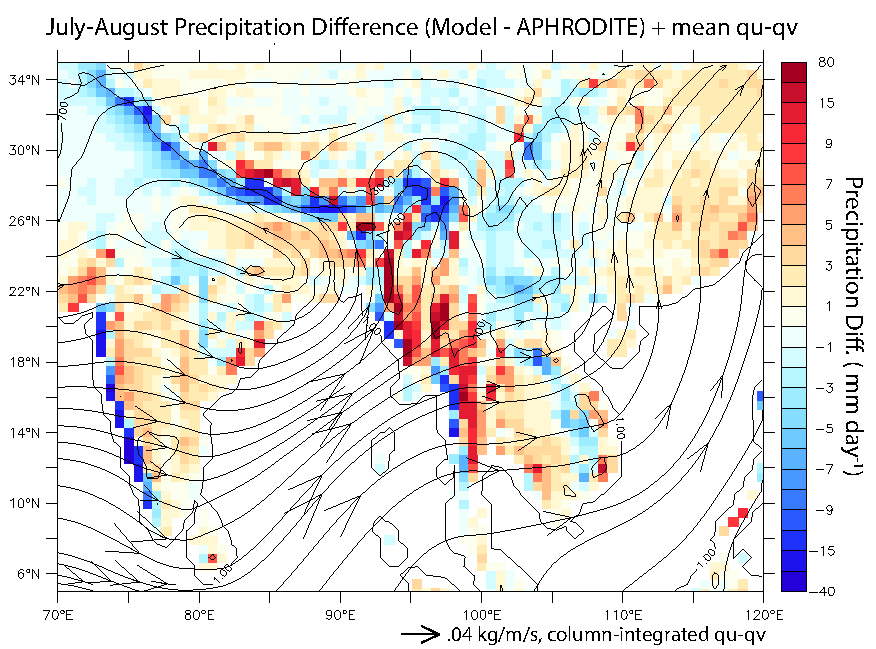
\includegraphics[width=36pc,angle=0]{figS2lmdzprecip}\\
  \caption{Discrepancy of LMDZ precipitation and observations from APHRODITE, July-August average.}\label{f14}
\end{figure}


%%%%%%%%%%%%%%%%%%%%%%%%%%%%%%%%%%%%%%%%%%%%%%%%%%%%%%%%%%%%%%%%%%%%%
% TABLES
%%%%%%%%%%%%%%%%%%%%%%%%%%%%%%%%%%%%%%%%%%%%%%%%%%%%%%%%%%%%%%%%%%%%%

\begin{table}[t]

\caption{All-Nepal Monsoon Rainfall for every July and August, 1951-2007, calculated as an area average over Nepal. Precipitation is in mm day$^{-1}$. The index is given by the monthly precipitation anomaly averaged over Nepal in units of standard deviation. Station quality improves dramatically starting in 1961 such that use of the 1951-1960 component is discouraged. 1961-2007 values are used to calculate monthly average and standard deviation. July: 11.34 mm day$^{-1}$ mean, st. dev. of 1.71 mm day$^{-1}$; in August, 9.91 mean, st. dev. of 1.54 mm day$^{-1}$. The inaccuracy of the index from 1951 to 1960 is reflected by the relatively high standard deviation of those points.}\label{t3}
\begin{center}
\begin{tabularx}{1\textwidth}{ >{\setlength\hsize{.1733\hsize}\centering}X >{\setlength\hsize{.08\hsize}\centering}X >{\setlength\hsize{.08\hsize}\centering}X  >{\setlength\hsize{.1733\hsize}\centering}X >{\setlength\hsize{.08\hsize}\centering}X >{\setlength\hsize{.08\hsize}\centering}X >{\setlength\hsize{.1733\hsize}\centering}X >{\setlength\hsize{.08\hsize}\centering}X >{\setlength\hsize{.08\hsize}\centering}X}
Month & Precip & Index & Month & Precip & Index & Month & Precip & Index \tabularnewline
\hline
\textit{July 1951} & \textit{7.46} & \textit{-2.27}  & July 1970 & 12.85 & 0.88 & July 1989 & 12.79 & 0.85 \tabularnewline
\textit{Aug 1951} & \textit{8.27} & \textit{-1.07}  & Aug 1970 & 8.40 & -0.98 & Aug 1989 & 9.30 & -0.40 \tabularnewline
\textit{July 1952} & \textit{6.09} & \textit{-3.07}  & July 1971 & 9.04 & -1.34 & July 1990 & 12.96 & 0.95 \tabularnewline
\textit{Aug 1952} & \textit{11.58} & \textit{1.08}  & Aug 1971 & 9.53 & -0.25 & Aug 1990 & 9.74 & -0.11 \tabularnewline
\textit{July 1953} & \textit{17.91} & \textit{3.84}  & July 1972 & 11.35 & 0.01 & July 1991 & 8.12 & -1.88 \tabularnewline
\textit{Aug 1953} & \textit{5.96} & \textit{-2.57}  & Aug 1972 & 6.62 & -2.14 & Aug 1991 & 10.99 & 0.70 \tabularnewline
\textit{July 1954} & \textit{13.68} & \textit{1.37}  & July 1973 & 8.23 & -1.82 & July 1992 & 9.19 & -1.26 \tabularnewline
\textit{Aug 1954} & \textit{10.49} & \textit{0.38}  & Aug 1973 & 8.92 & -0.65 & Aug 1992 & 9.24 & -0.44 \tabularnewline
\textit{July 1955} & \textit{7.45} & \textit{-1.60}  & Aug 1974 & 10.79 & 0.57 & Aug 1993 & 11.46 & 1.01 \tabularnewline
\textit{July 1956} & \textit{7.13} & \textit{-2.46}  & July 1975 & 12.98 & 0.96 & July 1994 & 9.51 & -1.07 \tabularnewline
\textit{Aug 1956} & \textit{9.95} & \textit{0.02}  & Aug 1975 & 8.61 & -0.85 & Aug 1994 & 10.09 & 0.12 \tabularnewline
\textit{July 1957} & \textit{12.72} & \textit{0.81}  & July 1976 & 9.36 & -1.16 & July 1995 & 10.76 & -0.34 \tabularnewline
\textit{Aug 1957} & \textit{8.54} & \textit{-0.89}  & Aug 1976 & 10.26 & 0.23 & Aug 1995 & 10.89 & 0.64 \tabularnewline
\textit{July 1958} & \textit{8.58} & \textit{-1.61}  & July 1977 & 10.14 & -0.70 & July 1996 & 12.41 & 0.63 \tabularnewline
\textit{Aug 1958} & \textit{14.77} & \textit{3.16}  & Aug 1977 & 10.31 & 0.26 & Aug 1996 & 11.22 & 0.85 \tabularnewline
\textit{July 1959} & \textit{8.23} & \textit{-1.82}  & July 1978 & 12.66 & 0.77 & July 1997 & 10.67 & -0.39 \tabularnewline
\textit{Aug 1959} & \textit{7.02} & \textit{-1.88}  & Aug 1978 & 8.79 & -0.73 & Aug 1997 & 9.48 & -0.28 \tabularnewline
\textit{July 1960} & \textit{11.05} & \textit{-0.17}  & July 1979 & 11.60 & 0.15 & July 1998 & 13.51 & 1.27\tabularnewline
\textit{Aug 1960} & \textit{8.54} & \textit{-0.89}  & Aug 1979 & 8.51 & -0.91 & Aug 1998 & 13.83 & 2.55 \tabularnewline
July 1961 & 9.59 & -1.02 & July 1980 & 12.46 & 0.66 & July 1999 & 11.19 & -0.09 \tabularnewline
Aug 1961 & 12.47 & 1.66 & Aug 1980 & 9.46 & -0.29 & Aug 1999 & 11.54 & 1.06 \tabularnewline
July 1962 & 9.79 & -0.91 & July 1981 & 13.06 & 1.01 & July 2000 & 11.01 & -0.19 \tabularnewline
Aug 1962 & 13.45 & 2.30 & Aug 1981 & 9.44 & -0.31 & Aug 2000 & 11.48 & 1.02 \tabularnewline
July 1963 & 10.90 & -0.26 & July 1982 & 9.22 & -1.24 & July 2001 & 10.90 & -0.26 \tabularnewline
Aug 1963 & 11.67 & 1.14 & Aug 1982 & 9.70 & -0.14 & Aug 2001 & 10.15 & 0.15 \tabularnewline
July 1964 & 13.43 & 1.22 & July 1983 & 10.78 & -0.33 & July 2002 & 12.18 & 0.49 \tabularnewline
Aug 1964 & 8.84 & -0.70 & Aug 1983 & 9.41 & -0.33 & Aug 2002 & 9.41 & -0.33 \tabularnewline
July 1965 & 10.25 & -0.64 & July 1984 & 14.45 & 1.82 & July 2003 & 12.97 & 0.95 \tabularnewline
Aug 1965 & 10.25 & 0.22 & Aug 1984 & 7.32 & -1.69 & Aug 2003 & 9.41 & -0.33 \tabularnewline
July 1966 & 9.78 & -0.91 & July 1985 & 13.45 & 1.23 & July 2004 & 12.73 & 0.81 \tabularnewline
Aug 1966 & 11.88 & 1.28 & Aug 1985 & 9.65 & -0.17 & Aug 2004 & 7.41 & -1.63 \tabularnewline
July 1967 & 11.40 & 0.04 & July 1986 & 11.44 & 0.06 & July 2005 & 10.14 & -0.70 \tabularnewline
Aug 1967 & 8.72 & -0.78 & Aug 1986 & 7.82 & -1.36 & Aug 2005 & 10.19 & 0.18 \tabularnewline
July 1968 & 10.93 & -0.24 & July 1987 & 13.36 & 1.18 & July 2006 & 9.16 & -1.27 \tabularnewline
Aug 1968 & 8.58 & -0.87 & Aug 1987 & 10.87 & 0.62 & Aug 2006 & 7.78 & -1.39 \tabularnewline
July 1969 & 9.94 & -0.82 & July 1988 & 14.52 & 1.86 & July 2007 & 13.67 & 1.36 \tabularnewline
Aug 1969 & 9.97 & 0.04 & Aug 1988 & 12.38 & 1.60 & Aug 2007 & 9.68 & -0.15 \tabularnewline
\end{tabularx}
\end{center}
\end{table}

\end{document}